\chapter{Gr\"ober Basis and Algebraic Geometry} \label{ch:ideals}
This chapter reviews fundamental concepts of commutative and 
computer algebra which are used in this work. 
Specifically, this chapter covers monomial ordering, polynomial ideals and 
varieties, and the computation of \Grobner bases.
It also overviews elimination theory as well as Hilbert's Nullstellensatz 
theorems and how
they apply to Galois fields. The results of these theorems are used in polynomial
abstraction and formal verification of Galois field circuits and 
are discussed 
in subsequent chapters. The material of this chapter is
mostly referred from the textbooks \cite{ideals:book} \cite{gb_book} and 
previous work by {\it Lv} \cite{lv:phd} as well as {\it Pruss} \cite{pruss:tcad15}.

\section{Algebraic Geometry Fundamentals}
\label{sec:geo}
\subsection{Monomials, Polynomials and Polynomial Arithmetics}
\begin{Definition} \label{def:mono}
A {\bf monomial} in variables $x_1,x_2,\cdots,x_d$ is a product of the form:
\begin{equation}
x_1^{{\alpha}_1} \cdot x_2^{{\alpha}_2} \cdot \cdots x_d^{{\alpha}_d},
\end{equation}
where $\alpha_i \ge 0, i\in\{1,\cdots,d\}$. 
The total degree of the monomial is $\alpha_{1}+\cdots+\alpha_{d}$.
\end{Definition} 

Thus, $x^2\cdot y$ is a monomial in variables $x,y$ with total degree $3$.
For simplicity, we will henceforth denote a 
monomial $x_1^{{\alpha}_1} \cdot x_2^
{{\alpha}_2} \cdot \cdots x_d^{{\alpha}_d}$ as $x^{\alpha}$, 
where $\alpha=({\alpha}_1,\cdots,{\alpha}_d)$ is a vector size $d$ of 
integers $\ge 0$, i.e., $\alpha \in \mathbb{Z}_{\ge 0}^{d}$.

\begin{Definition}\label{def:poly}
Let $\mathbb{R}$ be a ring. A {\bf polynomial} over $\mathbb{R}$ in the 
indeterminate $x$ is an expression of the form:
\begin{equation} \label{eq:poly1}
a_0 + a_1 x + a_2 x^2 + \cdots + a_k x^k = \sum_{i=0}^{k} a_i x^i, \forall a_i \in \mathbb{R}. 
\end{equation}

\end{Definition}

The constants $a_i$ are the coefficients and $k$ is the degree of the polynomial. 
For example, $8x^3 + 6x + 1$ is a polynomial in $x$ over $\mathbb{Z}$, with
coefficients $8$, $6$, and $1$ and degree $3$. 

\begin{Definition}
The set of all polynomials in the indeterminate
$x$ with coefficients in the ring $\mathbb{R}$ forms a {\bf
ring of polynomials} $\mathbb{R}[x]$. 
Similarly, $\mathbb{R}[x_1,x_{2},\cdots, x_{n}]$ 
represents the ring of multivariate polynomials with coefficients in $\mathbb{R}$.
\end{Definition}

For example, $\mathbb{Z}_{2^4}[x]$ stands for the set of all polynomials in
$x$ with coefficients in $\mathbb{Z}_{2^4}$. $8x^3 + 6x + 1$ is an instance 
of a polynomial contained in $\mathbb{Z}_{2^4}[x]$.

\begin{Definition}
A {\bf multivariate polynomial} $f$ in variables $x_1, x_2, \ldots, x_d$ 
with coefficients in any given field $\F$ is a finite linear 
combination of monomials with coefficients in $\F$: 
\begin{equation}
	f=\sum_{\alpha}a_{\alpha}\cdot x^{\alpha}, ~~a_{\alpha}\in \F \nonumber
\end{equation}

The set of all polynomials in $x_1, x_2, \ldots, x_d$ with coefficients in 
field $\F$ is denoted by $\F[x_1, x_2, \ldots, x_d]$. 
Thus, $f \in \F[x_1, x_2, \ldots, x_d]$

\begin{enumerate}
\item We refer to the constant $a_{\alpha} \in \F$ as the 
{\bf coefficient} of the monomial $a_{\alpha} x^{\alpha}$.
\item If $a_{\alpha} \neq 0$, we call $a_{\alpha} x^{\alpha}$ a term of $f$.
\end{enumerate}
\end{Definition}

As an example, $2x^2+y$ is a polynomial with two terms $2x^2$ and $y$, with 
$2$ and $1$ as coefficients respectively. 
In contrast, $x+y^{-1}$ is not a polynomial because the exponent of $y$ is 
less than $0$.

Since a polynomial is a sum of its terms,
these terms have to be arranged unambiguously so that they can be 
manipulated in a consistent manner.
Therefore, we need to establish a concept of 
{\bf term ordering} (also called monomial ordering).
A term ordering, represented by $>$, defines how
terms in a polynomial are ordered.

Common term orderings are lexicographic ordering (LEX) and its variants: 
degree-lexicographic ordering (DEGLEX) and reverse degree-lexicographic ordering (DEGREVLEX).

A {\bf lexicographic ordering} (lex) is a total-ordering $>$ such that 
variables in the terms are lexicographically ordered, i.e. simply based on 
when the variables appear in the ordering.
Higher variable-degrees take 
precedence over lower degrees for equivalent variables (e.g. $a^3 > a^2$ due to $a \cdot a \cdot a > a \cdot a \cdot 1$).
\begin{Definition}
{\bf Lexicographic order:} Let $x_1 > x_2 > \dots > x_d$
lexicographically. Also let $\alpha = (\alpha_1, \dots, \alpha_d);
~\beta = (\beta_1, \dots, \beta_d) \in \mathbb{Z}^d_{\geq 0}$. Then we
have: 
\begin{equation}
x^{\alpha} > x^{\beta} \iff 
\begin{cases}
& \text{Starting  from the  left, the first co-ordinates of $\alpha_i, \beta_i$} \\
& \text{that are different satisfy $\alpha_i > \beta_i$}

\end{cases}
\end{equation}
\end{Definition}

A {\bf degree-lexicographic ordering} (deglex) is a total-ordering $>$ such 
that the total degree of a term takes precedence over the lexicographic 
ordering.  
A {\bf degree-reverse-lexicographic ordering} (degrevlex) is the same as a
deglex ordering, however terms are lexed in reverse.

\begin{Definition}
{\bf Degree Lexicographic order:} Let $x_1 > x_2 > \dots > x_d$
lexicographically. Also let $\alpha = (\alpha_1, \dots, \alpha_d);
~\beta = (\beta_1, \dots, \beta_d) \in \mathbb{Z}^d_{\geq 0}$. Then we
have: 
\begin{equation}
x^{\alpha} > x^{\beta} \iff 
\begin{cases}
\sum_{i=1}^{d}\alpha_i > \sum_{i=1}^{d} \beta_i & \text{ or }\\
\sum_{i=1}^{d}\alpha_i = \sum_{i=1}^{d} \beta_i  \text{ and }
x^{\alpha} > x^{\beta} & \text{w.r.t. lex order}
\end{cases}
\end{equation}
\end{Definition}


\begin{Definition}
{\bf Degree Reverse Lexicographic order:} Let $x_1 > x_2 > \dots > x_d$
lexicographically. Also let $\alpha = (\alpha_1, \dots, \alpha_d);
~\beta = (\beta_1, \dots, \beta_d) \in \mathbb{Z}^d_{\geq 0}$. Then we
have: 
\begin{equation}
x^{\alpha} > x^{\beta} \iff 
\begin{cases}
\sum_{i=1}^{d}\alpha_i > \sum_{i=1}^{d} \beta_i  \text{ or }\\
\sum_{i=1}^{d}\alpha_i = \sum_{i=1}^{d} \beta_i  \text{ and the first co-ordinates}\\
\text{$\alpha_i, \beta_i$ from the right, which are different, satisfy $\alpha_i < \beta_i$}
\end{cases}
\end{equation}

\end{Definition}

Based on the {\it monomial ordering}, we have the following concepts:

\begin{Definition}
The {\bf leading term} is the first term in a term-ordered polynomial.
Likewise, the {\bf leading coefficient} is the coefficient of
the leading term. 
Finally, a {\bf leading monomial} is the leading term 
lacking the coefficient.  We use the following notation:
\begin{eqnarray}
     lt(f)&& \text{--- Leading Term} \\
     lc(f)&& \text{--- Leading Coefficient} \\
     lm(f)&& \text{--- Leading Monomial} \\
     tail(f)&& f - lt(f)
\end{eqnarray}
\end{Definition}

\begin{Example}
\begin{eqnarray}
     f      &=& 3a^2b + 2ab + 4bc \\
     lt(f)  &=& 3a^2b \\
     lc(f)  &=& 3 \\
     lm(f)  &=& a^2b \\
     tail(f) &=& 2ab+4bc
\end{eqnarray}
\end{Example}

{\bf Polynomial division} is an operation over polynomials that is dependent on
the imposed monomial ordering. Dividing a polynomial $f$ by another polynomial
$g$ cancels the leading term of $f$ to derive a new polynomial. 

\begin{Definition}
Let $\F$ be a field and let $f, g \in \F[x_1, x_2, \ldots, x_d]$ be polynomials
over the field. {\bf Polynomial division} of $f$ by $g$ is computes following:
\begin{equation}
f-\frac{lt(f)}{lt(g)}\cdot g
\end{equation}
This polynomial division is denoted
\begin{equation}
f\xrightarrow{g} r
\end{equation}
where $r$ is the resulting polynomial of the division.
If $\frac{lt(f)}{lt(g)}$ is non-zero, then $f$ is considered divisible by $g$, 
i.e. $g \mid f$.
\end{Definition}
Notice that if $g \nmid f$, that is if $f$ is not divisible by $g$,
then the division operation gives $r = f$.
\begin{Example}
Over $\R[x,y,z]$, set the lex term order $x > y > z$.
Let $f = -2x^3 + 2x^2yz + 3xy^3$ and $g = x^2+yz$.
\begin{equation}
\frac{lt(f)}{lt(g)} = \frac{-2x^3}{x^2} = -2x
\end{equation}
Since $\frac{lt(f)}{lt(g)}$ is non-zero $g|f$. The division, $f\xrightarrow{g} r$, 
is computed as:
\begin{eqnarray}
r &=& f-\frac{lt(f)}{lt(g)}\cdot g = -2x^3 + 2x^2yz + 3xy^3 - (-2x \cdot (x^2+yz)) \nonumber \\
&=& -2x^3 + 2x^2yz + 3xy^3 - (-2x^3-2xyz) = 2x^2yz + 3xy^3 + 2xyz
\end{eqnarray}
Notice that the division $f\stackrel{g}{\textstyle\longrightarrow}r$ cancels the leading term of $f$.
\end{Example}

Similarly, we can also define when a polynomial is divided (reduced) by a set of polynomials.
\begin{Definition}
    The {\bf reduction} of a polynomial $f$, by another polynomial $g$, to
    a reduced polynomial $r$ is denoted:
    \begin{equation*}
        f\stackrel{g}{\textstyle\longrightarrow}_{+}r
    \end{equation*}
    which is transitive and reflective closure of relation $f\stackrel{g}{\textstyle\longrightarrow}r$. 
    Reduction is carried out using multivariate, polynomial long division. 
    % The long division is performed according to a term-ordering on polynomials, and the division algorithm 
    %terminates when the leading term of the divisor does not divide any 
    %other term in the dividend.
  
    For sets of polynomials, the notation 
    \begin{equation*}
    f\stackrel{F}{\textstyle\longrightarrow}_+r    
    \end{equation*}
    represents the reduced polynomial $r$ resulting from $f$ as reduced by a 
    set of non-zero polynomials $F = \{f_1,\dots,f_s\}$.  The polynomial $r$ is considered {\bf reduced} if 
    $r = 0$  or no term in $r$ is divisible  by $lm(f_i), \forall f_i \in F$.
\end{Definition}

The reduction process $f\stackrel{F}{\textstyle\longrightarrow}_+r$, of 
dividing a polynomial $f$ by a set of polynomials of $F$, can be modeled as
repeated long-division of $f$ by each of the polynomials in $F$ until no
further reductions can be made. The result of this process is then $r$.
This reduction process is shown in Algorithm \ref{alg:polydiv}.

\begin{algorithm}[H]
\SetAlgoNoLine

 \KwIn{$f,f_{1},\dots,f_{s}$}
 \KwOut{$r,a_{1},\dots,a_{s}$, such that $f=a_{1}\cdot f_{1}+\dots+a_{s}\cdot f_{s}+r$.}
 
 $a_{1}=a_{2}=\dots=a_{s}=0$; $r=0$\;
 $p:=f$\;
 
 \While { $p \neq 0$ }
 {
	i=1\;
	divisionmark = false\;
	\While { $i\le s  $ \&\& divisionmark = false }
	{
		\eIf {$f_{i}$ can divide $p$}
		{
			$a_{i}=a_{i}+lt(p)/lt(f_{i})$\;
			$p=p-lt(p)/lt(f_{i}) \cdot f_{i}$\;
			divisionmark = true\;
		}
		{
			i=i+1\;
		}
	}
	
	\If {divisionmark = false}
	{
		$r=r+lt(p)$\;
		$p=p-lt(p)$\;
	}

 }
\caption{Polynomial Reduction}\label{alg:polydiv}
\end{algorithm}

The reduction algorithm keeps canceling the leading terms of polynomials 
until no more leading terms can be further canceled.
So the key step is $p=p-lt(p)/lt(f_{i}) \cdot f_{i}$, as the following 
example shows.
\begin{Example}
Given $f = y^{2}-x$ and $f_{1} = y - x$ in $\mathbb{Q}[x,y]$ with $deglex$: 
$y>x$, perform $f\stackrel{f_1}{\textstyle\longrightarrow}_+r$:

\begin{enumerate}
\item $f=y^{2}-x$, $f/f_{1}=f-lt(f)/lt(f_{1}) \cdot f_{1}=y^{2}-x-(y^{2} /y) \cdot (y-x)=y\cdot x-x$
\item $f=y\cdot x-x$, $f/f_{1}=f-lt(f)/lt(f_{1}) \cdot f_{1}=(y\cdot x-x)/f_{1}=x^{2}-x$
\item $f=x^{2}-x$, no more operations possible, so $r=x^{2}-x$
\end{enumerate}
\end{Example}

\subsection{Varieties and Ideals}
%%%%%%%%%%%%%%%%%%%%%%%%%%%%%%%%%%%%%%%%%%%%%%%%%%%%%%%%%%%%%%%%%%%%%%%%%%%%
%%%%%%%%%%%%%%%%%%%%%  variety %%%%%%%%%%%%%%%%%%%%%%%%%%%%%%%%%%%%%%%%%%
In computer-algebra based formal verification,
it is often necessary to analyze the presence 
or absence of solutions to a given system of constraints.
In our applications, these constraints are polynomials and their solutions 
are modeled as {\bf varieties}.

\begin{Definition}
Let $\F$ be a field, and let $f_1, \ldots, f_s 
\in \F[x_1, x_2, \ldots, x_d]$. 
We call $V(f_1, \dots, f_s)$ the {\bf affine variety} 
defined by $f_1, \dots, f_s$ as:
\begin{equation}
V(f_1, \ldots, f_s)= \{(a_1, \ldots, a_{d})\in \F^d:f_i(a_1, \ldots, a_d)=0, \forall{i},1\le i \le s\}
\end{equation}
\end{Definition}

$V(f_1, \dots, f_s)\in \F^d$ is {\bf the set of all solutions} in $\F^d$ 
of the system of equations: 
$f_1(x_1,\ldots,x_d)=\dots=f_s(x_1,\dots,x_d)=0$. 

\begin{Example}
Given $\mathbb{R}\left[x,y\right]$, $V(x^2+y^2)$ is the set of all elements
that satisfy $x^2+y^2=0$ over $\mathbb{R}^2$. So $V(x^2+y^2)=\{(0,0)\}$. 
Similarly, in $\mathbb{R}\left[x,y\right]$, $V(x^2+y^2-1)=\{all\  points\  on\ the\ circle: x^2+y^2-1=0\}$.
Note that varieties depend on which field we are operating on. 
For the same polynomial $x^2+1$, we have:
\begin{itemize}
\item In $\mathbb{R}[x]$, $V(x^2+1)=\emptyset$.
\item In $\mathbb{C}[x]$, $V(x^2+1)=\{(\pm i)\}$.
\end{itemize}
\end{Example}

The above example shows the variety can be infinite, finite (non-empty set) 
or empty. It is interesting to note that since we will be operating over
finite fields $\F_{q}$, and any finite set of points is a variety. Likewise,
any variety over $\F_{q}$ is finite (or empty).
Consider the points $\{(a_1,\dots, a_d): a_1, \dots, a_d \in \F_q\}$
in $\F_q^d$. Any single point is a variety of some polynomial system:
e.g. $(a_1,\dots, a_d)$ is a variety of $x_1-a_1 = x_2 - a_2 = \dots =
x_d-a_d=0$. {\bf Finite unions} and {\bf finite  intersections} of
varieties are also varieties. 

\begin{Example}
Let $U = V(f_1, \dots, f_s)$ and $W =
V(g_1, \dots, g_t)$ in $\F_{q}$. Then:  
\begin{itemize}
\item $U \cap W = V(f_1, \dots, f_s, g_1, \dots, g_t)$
\item $U \cup W = V(f_i g_j: 1 \leq i \leq s, 1 \leq j \leq t)$
\end{itemize}
\end{Example}

One important distinction we need to make about varieties is that a
variety depends not just on the given system of polynomial 
equations, but rather on the {\bf ideal} generated by the polynomials.

%%%%%%%%%%%%%%%%%%%%%  ideal %%%%%%%%%%%%%%%%%%%%%%%%%%%%%%%%%%%%%%%%%%
\begin{Definition} 
A subset $I \subset \F[x_1, x_2, \ldots, x_d]$ is an {
\bf ideal} if it satisfies:
\begin{itemize}
\item $0 \in I$
\item $I$ is closed under addition: $x, y \in I \Rightarrow x+y \in I$
\item If $x \in \F[x_1, x_2, \ldots, x_d]$ and $y \in I$, then $x\cdot y \in I$ and $y\cdot x \in  I$.
\end{itemize}
\end{Definition}

An ideal is generated by its {\it basis} or {\it generators}.

%%%%%%%%%%%%%%%%%%%%%  ideal basis%%%%%%%%%%%%%%%%%%%%%%%%%%%%%%%%%%
\begin{Definition}
Let $f_1, f_2, \ldots, f_s$ be 
polynomials of the ring $\F[x_1, x_2, \ldots, x_d]$. 
Let $I$ be an ideal generated by $f_1, f_2, \ldots, f_s$. Then:
\begin{equation}
I = \langle f_1,\dots,f_s \rangle=\{h_1 f_1 + h_2 f_2 + \ldots + h_s f_s : h_1,\dots,h_s\in\F[x_1, \dots, x_d]\} \nonumber
\end{equation}
then, $f_1, \ldots, f_s$ are called the {\bf basis (or generators)} of the 
ideal $I$ and correspondingly $I$ is denoted as $I = \langle f_1, f_2, 
\ldots, f_s \rangle$. 
\end{Definition}

\begin{Example}
The set of even integers, which is a subset of the ring of integers
$Z$, forms an ideal of $Z$. This can be seen from the following;
\begin{itemize}
\item $0$ belongs to the set of even integers.
\item The sum of two even integers $x$ and $y$ is always an even
  integer.
\item The product of any integer $x$ with an even integer $y$ is
  always an even integer.
\end{itemize}
\end{Example}

\begin{Example}
Given $\mathbb{R}\left[x,y\right]$, $I = \langle x, y \rangle$ is an 
ideal containing all polynomials generated by $x$ and $y$, 
such as $x^2+y$ and $x+x\cdot y$. The ideal
$J = \langle x^2, y^2 \rangle$ is an ideal containing all polynomials 
generated by $x^2$ and $y^2$, such as $x^2+y^3$ and $x^{10}+x^2\cdot y^2$. 
Notice that $J\subset I$ because every polynomial generated by $J$ can
be generated by $I$. 
But $I\neq J$ because $x+y$ can only be generated by $I$.
\end{Example}

The same ideal may have many different bases.
For instance, it is possible to have different sets of polynomials
$\{f_1,\dots,f_{s}\}$ and $\{g_{1},\dots,g_{t}\}$ that may generate the same 
ideal, i.e., 
$\langle f_{1},\dots,f_{s}\rangle=\langle g_{1},\dots,g_{t}\rangle$. Since 
variety depends on the ideal, these sets of polynomials have the same 
solutions.

\begin{Proposition}
If $f_1,\dots,f_{s}$ and $g_{1},\dots,g_{t}$ are bases of the same ideal 
in $\mathbb{F}[x_{1},\dots,x_{d}]$,
so that $\langle f_{1},\dots,f_{s}\rangle=\langle g_{1},\dots,g_{t}\rangle$, 
then $V(f_{1},\dots,f_{s})=V(g_{1},\dots,g_{t})$.
\end{Proposition}

\begin{Example}
	Consider the two bases $F_{1}=\{(2x^{2}+3y^{2}-11,x^{2}-y^{2}-3\}$ and $F_{2}=\{x^{2}-4,y^{2}-1\}$.
	These two bases generate the same ideal, i.e., $\langle F_{1}\rangle= \langle F_{2} \rangle$.{}
	Therefore, they represent the same variety, i.e., 
	\begin{equation}
		V(F_{1})= V( F_{2})=\{\pm 2, \pm 1\}.
	\end{equation}
\end{Example}

Ideals and their varieties are a key part of computer-algebra based formal
verification. A given hardware design can be transformed into a set
of polynomials over a field, $f_1, \ldots, f_s \in F$.
This set of polynomials gives the system of equations:
\begin{eqnarray}
f_1 = 0 \nonumber \\
\vdots \nonumber \\
f_s = 0 \nonumber
\end{eqnarray}
Using algebra, it is possible to derive new equations from the original 
system.
The ideal $\langle f_1,\ldots, f_s \rangle$ provides a way of analyzing 
such {\it consequences} of a system of polynomials.

\begin{Example}
Given two equations in $\mathbb{R}[x,y,z]$:
\begin{eqnarray}
x=z+1 \nonumber \\
y=x^2+1 \nonumber 
\end{eqnarray}
we can eliminate $x$ to obtain a new equation:
\begin{equation}
y=(z+1)^2+1=z^2+2z+2 \nonumber 
\end{equation}
Let $f_1, f_2, h \in \mathbb{R}[x,y,z]$ be polynomials based on these 
equations:
\begin{eqnarray}
f_1 &= x-z-1 &= 0 \nonumber \\
f_2 &= y-x^2-1 &= 0 \nonumber \\
h   &= y-z^2-2z-2 &= 0 \nonumber
\end{eqnarray}
If $I$ is the ideal generated by $f_1$ and $f_2$, i.e. 
$I=\langle f_1, f_2 \rangle$, then we find $h \in I$ as follows:
\begin{eqnarray}
g_1 &= x+z+1 \nonumber \\
g_2 &= 1     \nonumber \\
h &= g_1\cdot f_1+g_2\cdot f_2  = y-z^2-2z-2 \nonumber
\end{eqnarray}
where $g_1, g_2 \in \mathbb{R}[x,y,z]$.
Thus, we call $h$ a {\bf member of the ideal} $I$.
\end{Example}

%\subsection{Ideals of Varieties}

Let $\mathbb{F}$ be any field and let $\mathbf{a}=(a_{1},\dots,a_{d}) \in \mathbb{F}^d$ be a point, and $f \in
\mathbb{F}[x_1,\dots, x_d]$ be a polynomial. We say that $f$ {\it vanishes} on $\mathbf{a}$ if $f(\mathbf{a}) = 0$, i.e.,
$\mathbf{a}$ is in the variety of $f$.

\begin{Definition}
For any variety $V$ of $\mathbb{F}^d$, the ideal of polynomials that vanish on $V$,
called the {\it vanishing ideal of $V$}, is defined as {\bf ideal of variety}:
$$I(V) = \{f\in
\mathbb{F}[x_1,\dots, x_d]: \forall \mathbf{a} \in V, f(\mathbf{a}) =
0\}$$ 
\end{Definition}

\begin{Proposition}\label{pro:iofv}
	If a polynomial $f$ vanishes on a variety $V$, then $f \in I(V)$. 
\end{Proposition}

\begin{Example}
	Let ideal $J=\langle x^{2},y^{2}\rangle$. Then $V(J)=\{(0,0)\}$.
	All polynomials in $J$ will obviously agree with the solution and vanish on this variety.
	However, the polynomials $x,y$ are not in $J$ but they also vanish on this variety. 
	Therefore, $I(V(J))$ is the set of all polynomials that vanish on $V(J)$, and the polynomials
	$x,y$ are members of $I(V(J))$.
\end{Example}

\begin{Definition}\label{def:radical}
Let $J \subset \mathbb{F}[x_1,\dots, x_d]$ be an ideal. The {\bf radical of $J$} is defined as $\sqrt{J} = \{f \in
\mathbb{F}[x_1,\dots, x_d]: \exists m \in \mathbb{N}, f^m \in J\}$. 
\end{Definition}

\begin{Example}
Let $J=\langle x^2,y^2\rangle \subset \mathbb{F}\left[x,y\right]$.
Neither $x$ nor $y$ belongs to $J$, but they belong to $\sqrt J$.
Similarly, $x\cdot y \notin J$, but since $(x \cdot y)^{2}=x^{2}\cdot y^{2}\in J$, therefore,
$x\cdot y \in \sqrt J$. 
\end{Example} 

When $J = \sqrt J$, then $J$ is said to be a 
{\it radical ideal}. Moreover, $I(V)$ is a radical ideal.
By analyzing the ideal $J$, generated by a system of polynomials derived 
from a hardware design, its variety $V(J)$, and the ideal of 
polynomials that vanish over this variety, $I(V(J))$, we can reason about the 
existence of certain properties of the design. To check for the validity of 
a property, we formulate the 
property as a polynomial and then perform an {\bf ideal membership test} to 
determine if this polynomial is contained within the ideal $I(V(J))$. 
A {\bf \Grobner basis} provides a decision procedure for performing this 
test, which is described in the following part. 

\subsection{\Grobner Bases}

As mentioned earlier, different polynomial sets may generate the same 
ideal. Some of these generating sets may be a better representation of 
the ideal, and thus provide more information and insight into the properties 
of the ideal. One such ideal representation is a {\bf \Grobner basis}, which has
a number of important properties that can solve numerous polynomial 
decision questions:

\begin{itemize}
\item Presence or absence of solutions (varieties)
\item Dimension of the varieties
\item Ideal membership of a polynomial
\item $\dots \dots$
\end{itemize} 

In essence, a \Grobner basis is a canonical representation of an ideal.
There are many equivalent definitions of \Grobner bases, so we start with 
the definition that best describes their properties:

\begin{Definition}
A set of non-zero polynomials $G=\{g_1,\dots,g_t\}$ which generate the 
ideal $I=\langle g_1,\dots,g_t\rangle$, is called a 
{\bf Gr\"obner basis} for $I$ if and only if 
for all $f \in I$ where $f \neq 0$, there exists a $g_i \in G$ such that $lm(g_i)$ divides $lm(f)$.
\begin{eqnarray}
G = \text{Gr\"obner{Basis}} (I) \iff 
\forall f \in I: f \neq 0, \exists g_i \in G: lm(g_i)\ |\ lm(f)
        \label{eqn:groebnermin}
    \end{eqnarray}
    
\end{Definition}

\Grobner basis has an important property, and therefore can be used to perform ideal membership test.
Formally speaking, a \Grobner basis gives a decision procedure to test 
for polynomial membership in an ideal. This is explained in the following 
Theorem.
    
\begin{Theorem}\label{the:membership}
	{\bf Ideal Membership Test}
 Let $G = \{g_1,\cdots,g_t \}$ be a Gr\"obner basis for an ideal $I \subset \mathbb{K}[x_1,\cdots,x_d ]$
	and let $f \in \mathbb{K}[x_{1},\dots, x_{d}]$. Then $f \in I$ if and only if the remainder on division of $f$ by
	$G$ is zero.
\end{Theorem}
In other words, 
\begin{equation}
f \in I \iff f \stackrel{G}{\textstyle\longrightarrow}_+0
\end{equation}

\begin{Example}
Consider Example \ref{exp:gbsimple}. Let $f = y^2x - x$ be another
polynomial. Note that $f = yf_1 + f_2$, so $f \in I$. If we divide $f$
by $f_1$ first and then by $f_2$, we will obtain a zero
remainder. However, since the set $\{f_1, f_2\}$ is not a Gr\"{o}bner
basis, we find that the reduction $f
\stackrel{f_2}{\textstyle\longrightarrow} x^2 - x
\stackrel{f_1}{\textstyle\longrightarrow} x^2 - x  \neq 0$;
i.e. dividing $f$ by $f_2$ first and then by $f_1$ does not lead to a
zero remainder. However,  if we compute the Gr\"{o}bner basis $G$ of
$I$, $G = \{x^2 - x, yx - y, y^2 - x\}$, dividing $f$ by polynomials
in $G$ in any order will always lead to the zero remainder. Therefore,
one can decide ideal membership unequivocally using the Gr\"{o}bner
basis. 
\end{Example}


The foundation for computing the \Grobner basis of an ideal was laid out 
by Buchberger\cite{buchberger_thesis}.
Given a set of polynomials $F=\{f_{1},\dots,f_{s}\}$ that generate ideal $I=
\langle f_{1},\dots,f_{s} \rangle$, 
Buchberger gives an algorithm to compute a Gr\"obner basis $G=\langle g_{1},
\dots,g_{t}\rangle$. This algorithm relies on the notions of $S$-polynomials 
and polynomial reduction.

\begin{Definition}
For $f, g \in \F[x_1,\dots,x_d]$, an {\bf S-polynomial} $Spoly(f,g)$ is 
defined as:
\begin{equation}
    Spoly(f,g)=\frac{L}{lt(f)}\cdot f - \frac{L}{lt(g)}\cdot g
    \label{eqn:spoly}
\end{equation}
\begin{equation}
\text{where }L = lcm\left(lt(f), lt(g)\right) \nonumber
\end{equation}
Note $lcm$ denotes least common multiple.
\end{Definition}

With the notions of $S$-polynomials and polynomial reduction in place,
we can now present Buchberger's Algorithm 
for computing Gr\"obner bases \cite{buchberger_thesis}. Note that a fixed 
monomial (term) ordering is required for a \Grobner basis 
computation to ensure that polynomials are manipulated in a consistent 
manner.

\begin{algorithm}[H]
\SetAlgoNoLine
 \KwIn{$F = \{f_1, \dots, f_s\}$, such that $I=\langle f_1, \dots, f_s\rangle$}, and term order $>$
 \KwOut{$G = \{g_1,\dots ,g_t\}$, a Gr\"{o}bner basis of $I$ }
  $G:= F$\;
  \Repeat{$G = G'$}
  {
  	$G' := G$\;
  	\For{ each pair $\{f_{i}, f_{j}\}, i \neq j$ in $G'$} 
	{
		$Spoly(f_{i}, f_{j}) \stackrel{G'}{\textstyle\longrightarrow}_+r$ \;
		\If{$r \neq 0$}
		{
			$G:= G \cup \{r\}$ \;
		}
	}
   }
\caption {Buchberger's Algorithm}\label{alg:gb}
\end{algorithm}

Buchberger's algorithm takes pairs of polynomials ($f_{i}, f_{j}$) in 
the basis $G$ and combines them into ``$S$-polynomials'' 
($Spoly(f_{i}, f_{j})$) to cancel leading terms. The $S$-polynomial is then 
reduced (divided) by all elements of $G$ to a remainder $r$, denoted as  
$Spoly(f_{i}, f_{j}) \stackrel{G}{\textstyle\longrightarrow}_+r$. This
process is repeated for all unique pairs of polynomials, including
those created by newly added elements, until no new polynomials are
generated; ultimately constructing the \Grobner basis.
\begin{Example}\label{exp:gbsimple}
Consider the ideal $I \subset \mathbb{Q}[x, y]$, $I = \langle f_1, f_2 
\rangle$, where $f_1 = yx - y, ~f_2 = y^2 - x$. 
Assume a degree-lexicographic term ordering with $y > x$ is imposed. 

First, we need to compute $Spoly(f_{1},f_{2})=x\cdot f_{2}-y\cdot f_{1}=y^{2}-x^{2}$.
Then we conduct a polynomial reduction 
$y^{2}-x^{2}\stackrel{f_{2}}{\textstyle\longrightarrow}x^{2}-x \stackrel{f_{1}}{\textstyle\longrightarrow}x^{2}-x$.
Let $f_{3}=x^{2}-x$. Then $G$ is updated as $\{f_{1},f_{2},f_{3}\}$. Next we compute $Spoly(f_{1},f_{3})=0$. So there
is no new polynomial generated. Similarly, we compute $Spoly(f_{2},f_{3})=x\cdot y^{2}-x^{3}$, followed by 
$x\cdot y^{2}-x^{3}\stackrel{f_{1}}{\textstyle\longrightarrow}y^{2}-x^{3} \stackrel{f_{2}}{\textstyle\longrightarrow}x-x^{3}
\stackrel{f_{2}}{\textstyle\longrightarrow}0$. Again, no polynomial is generated. Finally, $G=\{f_{1,}f_{2},f_{3}\}$.

\end{Example}

When computing a \Grobner basis, it's important to note that if $lt(f_i)$ 
and $lt(f_j)$ have no common variables, the S-poly reduction step in 
Buchberger's algorithm will reduce to 0.
\begin{Lemma}
In Buchberger's algorithm, when $gcd(lt(f_i),lt(f_j)) = 0$, the S-poly reduction
$$Spoly(f_{i}, f_{j}) \stackrel{G'}{\textstyle\longrightarrow}_+r$$
will produce $r=0$.
\end{Lemma}

\begin{Proof}
If $lt(f)$ and $lt(g)$ have no common variables,  
$L=lcm(lt(f),lt(g))=lt(f)\cdot lt(g)$. Then: 
\begin{equation}
    Spoly(f,g)=\frac{L}{lt(f)}\cdot f - \frac{L}{lt(g)}\cdot g=
\frac{lt(f)\cdot lt(g)}{lt(f)}\cdot f - \frac{lt(f)\cdot lt(g)}{lt(g)}\cdot g
= lt(g)\cdot f - lt(f)\cdot g \nonumber
\end{equation}
Thus, every monomial in $Spoly(f, g)$ is divisible by either $lt(f)$ 
or $lt(g)$, so computing 
$Spoly(f, g) \stackrel{f,g}{\textstyle\longrightarrow}_+r$ will give $r=0$.
\end{Proof}

A \Grobner basis is not a canonical representation of an ideal, but a
{\bf reduced \Grobner basis} is. To compute a reduced \Grobner basis, we
first must compute a minimal \Grobner basis.

\begin{Definition}\label{def:minigb}
A {\bf minimal Gr\"obner basis} for a polynomial ideal $I$ is a \Grobner basis $G$ for $I$ such that
	\begin{itemize}
		\item $lc(g_{i})=1,\forall g_{i}\in G$
		\item $\forall g_{i} \in G$,  $lt(g_{i}) \notin \langle lt(G-\{g_{i}\})\rangle$
	\end{itemize}
\end{Definition}
A {\bf minimal} \Grobner basis is a \Grobner basis such that all polynomials
have a coefficient of $1$ and no leading term of any element in $G$ divides 
another in $G$.
Given a \Grobner basis $G$, a minimal \Grobner basis can be
computed as follows:
\begin{enumerate}
\item Minimize every $g_i \in G$, i.e $g_i=g_i/lc(g_i)$
\item For $g_i, g_j \in G$ where $i\neq j$, remove $g_i$ from $G$ if $lt(g_i)\mid lt(g_j)$, i.e. remove every polynomial in $G$ whose leading term is divisible by the leading term of some other polynomial in $G$.
\end{enumerate}

A minimal Gr\"obner basis can then be further reduced.
\begin{Definition}
	A {\bf reduced Gr\"obner basis} for a polynomial ideal $I$ is a Gr\"obner basis $G=\{g_{1},\dots,g_{t}\}$ such that:
	\begin{itemize}
		\item $lc(g_{i})=1,\forall g_{i}\in G$
		\item $\forall g_{i} \in G$, no monomial of $g_{i}$ lies in $\langle lt(G-\{g_{i}\})\rangle$
	\end{itemize}
\end{Definition}
$G$ is a reduced Gr\"obner basis when no monomial of any element in $G$ 
divides the leading term of another element. 
This reduction is achieved as follows:

\begin{Definition}
Let $H = \{h_1, \ldots, h_t\}$ be a minimal Gr\"obner basis.  Apply
the following reduction process: 
\begin{itemize}
\item $h_1 \stackrel{G_1}{\textstyle\longrightarrow}_+ g_1$, where
  $g_1$ is reduced w.r.t. $G_1 = \{h_2, \ldots, h_t\}$

\item $h_2 \stackrel{G_2}{\textstyle\longrightarrow}_+ g_2$, where
  $g_2$ is reduced w.r.t. $G_2 = \{g_1, h_3, \ldots, h_t\}$
\item $h_3 \stackrel{G_3}{\textstyle\longrightarrow}_+ g_3$, where
  $g_3$ is reduced w.r.t. $G_3 = \{g_1, g_2, h_4, \ldots, h_t\}$

\hspace{0.25in} $\vdots$
\vspace{0.1in}
\item $h_t \stackrel{G_t}{\textstyle\longrightarrow}_+ g_t$, where
  $g_t$ is reduced w.r.t. $G_t = \{g_1, g_2, g_3, \ldots, g_{t-1}\}$
\end{itemize}
Then $G = \{g_1, \ldots, g_t\}$ is a {\bf reduced Gr\"obner basis.}
\end{Definition}


Subject to the given term order $>$, such a reduced Gr\"obner
  basis $G = \{g_1, \dots, g_t\}$ is a {\bf unique canonical
    representation of the ideal}, as 
given by Proposition \ref{pro:unique} below.


\begin{Proposition}\label{pro:unique} \cite{gb_book} 
Let $I \neq \{0\}$ be a polynomial ideal. Then, for a given monomial ordering, $I$ has a unique reduced Gr\"obner basis.
\end{Proposition}

% TODO discuss complexity

The high computational complexity if Gr\"obner basis computation is treated as an issue
because of its high cost on time and space. Concretely, for arbitrary polynomial set, 
the worst case computation time/space cost of its Gr\"obner basis is doubly exponential bounded -- $q^{q^{O(|\phi|)}}$
\cite{dube1986complexity}. However, in practice such as applications of circuit verification, 
the polynomial is well restricted rather than arbitrary.
Gao et al. \cite{gao:qe-gf-gb} proves that when the number of variables and degree of polynomials 
are restricted, the complexity reduces to single exponential $q^O(|\phi|)$.
This provides the possibility to make use of Gr\"obner basis under restricted situations,
which is the theoretic basis of this dissertation.

\Grobner basis computation depends on the $Spoly$ computation, which in turn 
depends on the leading terms of polynomials. Thus, different monomial 
orderings can result in different \Grobner basis computations for the 
same ideal. Computation using a degrevlex ordering tends to be least 
difficult, while lex ordering tends to be computationally complex. However, 
lex ordering used in the computation of \Grobner basis is an {\bf elimination
ordering}; that is, the polynomials contained in the resulting \Grobner basis
have continuously eliminated variables in the ordering. This is the topic of 
elimination theory, which is described in the following sections as well as 
its theoretic basis -- the Nullstellensatz theory.

\section{Hilbert's Nullstellensatz}

In this section, we further describe some correspondence between ideals and 
varieties in the context of algebraic geometry. The celebrated results of 
Hilbert's Nullstellensatz establish these correspondences.

%%%%%%%%%%%%%%%%%algebraically closed field%%%%%%%%%%%%%
\begin{Definition}\label{def:acf}
A field $\overline {\F}$ is an {\bf algebraically closed} field if every  
polynomial in one variable with degree at least $1$, with coefficients 
in $\overline {\F}$, has a root in $\overline {\F}$. 
\end{Definition}
In other words, any non-constant polynomial equation over 
$\overline {\F}\left[x\right]$ always has at least one root 
in $\overline {\F}$. Every field $\F$ is contained in an algebraically 
closed one $\overline {\F}$. 
For example, the field of real numbers $\mathbb{R}$ is not an algebraically closed 
field, because $x^2+1=0$ has no root in $\mathbb{R}$. 
However, $x^2+1=0$ has roots in the field of 
complex numbers $\mathbb{C}$, which is an algebraically closed field. 
In fact, $\mathbb{C}$ is the algebra closure of $\mathbb{R}$. 
Every algebraically closed field is an infinite field. 

%%%%%%%%%%%%%%%weak nullstellensatz%%%%%%%%%%%%%
\begin{Theorem}{Weak Nullstellensatz}
%$\left[\bf{Weak\  Nullstellensatz}\right]$ 
Let $J \subset \overline {\F}[x_1, x_2, \cdots, x_d]$ 
be an ideal satisfying $V(J)=\emptyset$. 
Then $J=\overline {\F}[x_1, x_2, \cdots, x_d]$, Or equivalently, 
\begin{equation}
V(J)=\emptyset\ \iff\ J=\overline {\F}[x_1, x_2, \cdots, x_d]=\langle 1 \rangle 
\end{equation}
\end{Theorem}

\begin{Corollary}
	Let $J=\langle f_{1},\dots,f_{s} \rangle \subset \overline {\F}[x_1, x_2, \cdots, x_d]$. 
	Let $G$ be the reduced Gr\"obner basis of $J$. Then $V(J)=0 \iff G=\{1\}$.
\end{Corollary}

{\bf Weak Nullstellensatz} offers a way to evaluate whether or not the 
system of multivariate polynomial equations (ideal $J$) has common solutions 
in ${\overline {\F}}^d$. For this purpose, we only need to check if 
the ideal is generated by the unit element, i.e., $1\in J$. 
This approach can be used to evaluate the feasibility of constraints in 
verification problems.
%%%%%%%%%%%%%%%%%%%%%%%%%strong Nullstellensatz%%%%%%%%%%%%%%%%%%%%%%%%%%%%%% 
An interesting result is one of {\bf Strong 
Nullstellensatz}.
The strong
Nullstellensatz establishes the correspondence between radical ideals
and varieties. 

\begin{Theorem}\label{thm:sns}
({\it The Strong Nullstellensatz} \cite{gb_book}) 
Let $\overline{\F}$ be an algebraically closed field, and let $J$
be an ideal in $\overline{\F}[x_1,\dots, x_d]$. 
Then we have $I(V_{\overline{\F}}(J)) =\sqrt{J}$. 
\end{Theorem}

%\subsection{Nullstellensatz over Galois fields}

Strong Nullstellensatz holds a special form over Galois fields $\Fq$.
Recall the notion of vanishing polynomials over Galois fields from the 
previous chapter: for every element $A \in \Fq$, $A-A^q = 0$; then the 
polynomial $x^q-x$ in $\Fq[x]$ vanishes over $\Fq$. Thus, if 
$J_0=\langle x^q-x \rangle$ is the ideal generated by the vanishing 
polynomial, $V(J_0)=\Fq$. Similarly, over $\Fq[x_1,\dots,x_d]$, $J_0$ is 
$\langle x_1^q-x_1,\dots,x_d^q-x_d \rangle$ and $V(J_0)=(F_q)^d$.


\begin{Definition}
Given two ideals, $I_1=\langle f_1, \dots,f_s \rangle$ and 
$I_2=\langle g_1,\dots g_t\rangle$, then the {\bf sum of ideals} 
$I_1+I_2=\langle f_1,\dots,f_s,g_1,\dots g_t\rangle$
\end{Definition}

\begin{Theorem}
({\it Strong Nullstellensatz over $\Fq$})
For any Galois field $\Fq$, let $J \subset \Fq[x_1,\dots,x_d]$ be any ideal 
and let $J_0 = \langle x_1^q-x_1, x_d^q-x_d \rangle$ be the ideal of all
vanishing polynomials. Let $V_{\Fq}(J)$ denote the variety of $J$ over $\Fq$.
Then, $I(V_{\Fq}(J))=J+J_0$.
\end{Theorem}

The proof is given in \cite{gao:gf-gb-ms}. Here, we provide a proof outline.

\begin{Proof}
\begin{enumerate}
\item $\sqrt{J+J_0} = J+J_0$. That is, $J+J_0$ is a radical ideal.
\item $V_{\Fq}(J)=V_{\overline{\Fq}}(J+J_0)$.
\item Due to (2), $I(V_{\Fq}(J)) = I(V_{\overline{\Fq}}(J+J_0))$. 
By Strong Nullstellensatz, this is equivalent to $\sqrt{J+J_0}$.
Finally, due to (1), this is equivalent to $J+J_0$.
\end{enumerate}
\end{Proof}


Using this result, Weak Nullstellensatz can be 
modified to be applicable over finite fields $\Fq$.
%%%%%%%%%%%%%%%%weak nullstellensatz in finite field%%%%%%%%%%%%%
\begin{Theorem}\label{wnull:ff}
$[\bf{Weak~Nullstellensatz~in~\Fq}]$\cite{null:1890}\\
Given $f_1,f_2,\cdots,f_s \in \Fq[x_1,x_2,\cdots,x_d]$. 
Let $J=\langle f_1,f_2,\cdots,f_s\rangle \subset \Fq[x_1,
x_2, \cdots, x_d]$ be an ideal. Let $J_0 = \langle 
x_1^{2^k}-x_1,x_2^{2^k}-x_2,\cdots,x_d^{2^k}-x_d \rangle$ be the ideal
of vanishing polynomials in $\Fq$. Then
$V_{\Fq}(J) = V_{\overline {\Fq}}(J +
J_0)=\emptyset$,  if and only if the reduced
Gr\"obnerBasis$(J+J_{0})=\{1\}$. 
\end{Theorem}

The proof is given in \cite{null:1890}. Here, we provide a proof outline.

\begin{Proof}
The variety of $J$ over $\Fq[x_1,x_2,\cdots,x_d]$ 
is equivalent to the variety over the algebraic closure of $\Fq$ 
intersected by the entire field $\Fq$. That is, $V_{\Fq}(J)=V_{\overline 
{\Fq}}(J) \cap \Fq$. 

Let $J_0 = \langle 
x_1^{2^k}-x_1,x_2^{2^k}-x_2,\cdots,x_d^{2^k}-x_d \rangle$ be the ideal
generated by all vanishing polynomials in $\Fq[x_1,x_2,\cdots,x_d]$.
Then $V_{\overline{\Fq}}(J_0)=\Fq$. 

Thus, $V_{\Fq}(J) = V_{\overline{\Fq}}(J)\cap V_{\overline{\Fq}}(J_0)
= V_{\overline{\Fq}}(J+J_0)$.
\end{Proof}


\section{Elimination and Abstraction Theory}
\label{sec:abstraction}
Elimination of certain variables in a system of polynomials is a common 
operation when some variables is not needed in modeling and analysis. 
In this section, eliminating variables targets a tight-bound over-approximation 
which is equivalent to existential quantifier elimination in first-order logic,
or variable smoothing in Boolean operations. We introduce a eliminating method 
based on algebraic geometry concepts, and use it as the fundamentals of 
abstraction of a circuit.

\subsection{Elimination Theory}
Assume we are given a set of polynomials $f_1,\dots,f_s$ belongs to ring $\Fq[x_1,\dots,x_l,\dots,x_d]$.
First, we show that eliminating the $x_1,\dots,x_l$ variables is equivalent to 
{\it projecting} the variety $V(\langle f_1,\dots,f_s\rangle)$ from 
$\Fq^d$ to $\Fq^{d-l}$. Figure \ref{fig:projection} is an example of projection in space of varieties
from $\Fq^3$ to $\Fq^2$, corresponding to eliminating variable $x_1$ from 
a system of polynomials belonging to $\Fq[x_1,x_2,x_3]$.

\begin{figure}[H]
\centering{
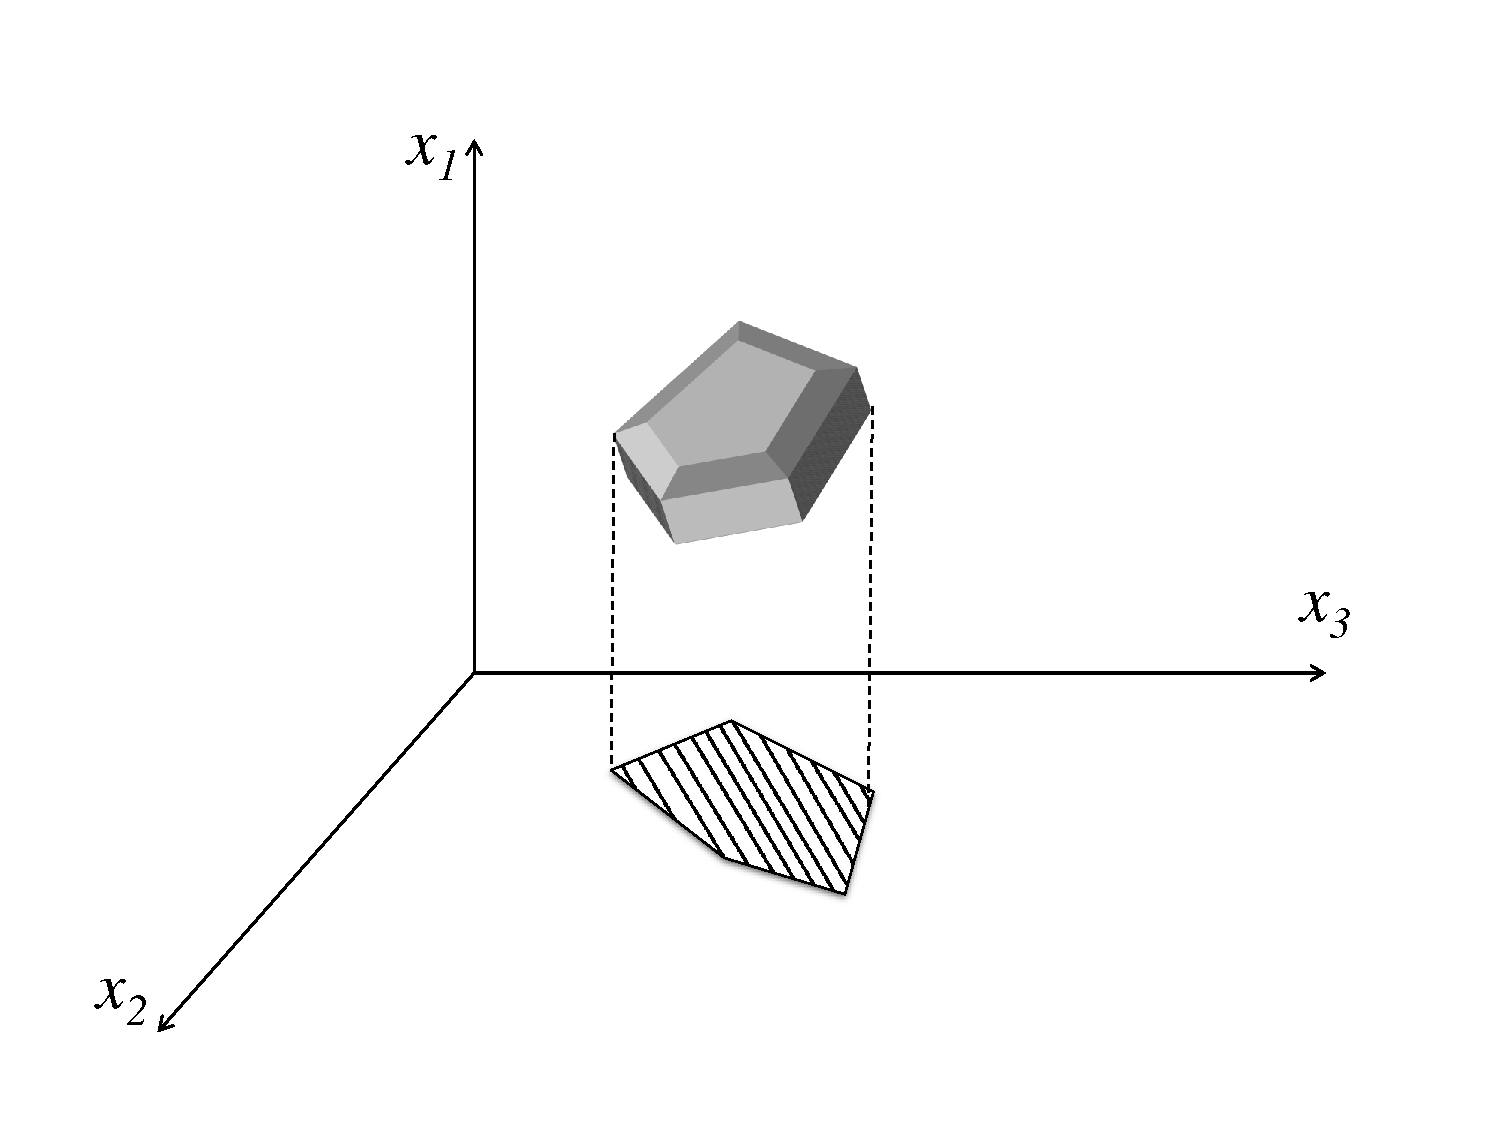
\includegraphics[width=\textwidth]{newfig/projection.pdf}
\caption{An example of projection from $\Fq^3$ to $\Fq^2$}
\label{fig:projection}}
\end{figure}

Formally, we define concepts of projection and elimination ideal:
\begin{Definition}
The {\bf $l$-th projection} mapping is defined as:
$$\pi_l:\Fq^d\to\Fq^{d-l},~~\pi_l((x_1,\dots,x_d)) = (x_{l+1}.\dots,x_d)$$
where $l<d$. For any set $A \subseteq \Fq^d$, we write 
$$\pi_l(A) = \{\pi_i(x):x\in A\}\subseteq \Fq^{d-l}$$
\end{Definition}

\begin{Definition}
Let $J$ be an ideal in  $\Fq[x_1,\dots,x_d]$. The $l$-th 
{\bf elimination ideal} $J_l$ is the ideal of $\Fq[x_{l+1},\dots,x_d]$ defined
by
\begin{equation}
J_l = J \cap \Fq[x_{l+1},\dots,x_d]
\end{equation}
\end{Definition}

The elimination ideal $J_l$ has eliminated all the variables 
$x_1,\dots,x_l$, i.e. it only contains polynomials with variables in
$x_{l+1},\dots,x_d$. 
This shows that in finite fields, projection of the variety $V_{d}(\langle f_1,\dots,f_s\rangle)$
from $\Fq^d$ to $\Fq^{d-l}$, is exactly the variety $V_{d-l}(\langle f_1,\dots,f_s\rangle\cap \Fq[x_{l+1},\dots,x_d])$.

Elimination theory uses {\bf elimination ordering} 
to systematically eliminate variables from a system of polynomial
equations.
We can generate elimination ideals by computing
\Grobner bases using elimination orderings. 

\begin{Theorem}{Elimination Theorem}
%$\left[\bf{Elimination\  Theorem}\right]$
Let $J$ be an ideal in $\F[x_1,\dots,x_d]$ and let $G$ be the \Grobner 
basis of $J$ with respect to the lex order (elimination order) 
$x_1>x_2>\dots>x_d$. Then, for every $0\leq l\leq d$,
\begin{equation}
G_l=G\cap \F[x_{l+1},\dots,x_d]
\end{equation}
is a \Grobner basis of the $l$-th elimination ideal $J_l$.
\label{thm:elimth}
\end{Theorem}

This can be better understood using the following example.

\begin{Example}
Given the following equations in $\R[x,y,z]$
\begin{eqnarray}
x^2+y+z&=1 \nonumber \\
x+y^2+z&=1 \nonumber \\
x+y+z^2&=1 \nonumber
\end{eqnarray}
let $I$ be the ideal generated by these equations:
\begin{equation}
I=\langle x^2+y+z-1, x+y^2+z-1, x+y+z^2-1\rangle \nonumber
\end{equation}
The \Grobner basis for $I$ with respect to lex order $x>y>z$ is 
found to be $G=\{g_1,g_2,g_3,g_4\}$ where
\begin{eqnarray}
g_1&=&x+y+z^2-1 \nonumber \\
g_2&=&y^2-y-z^2+z \nonumber \\
g_3&=&2yz^2+z^4-z^2 \nonumber \\
g_4&=&z^6-4z^4+4z^3-z^2 \nonumber
\end{eqnarray}

Notice that while $g_1$ has variables in $\R[x,y,z]$, $g_2$ and $g_3$ only 
have variables in $\R[y,z]$ and $g_4$ only has variables in $\R[z]$. Thus, 
$G_1=G\cap \R[y,z]=\{g_2,g_3,g_4\}$ and $G_2=G\cap \R[z]=\{g_4\}$

Also notice that since $g_4$ only contains variable $z$, and since $g_4=0$, 
a solution for $z$ can be obtained. This solution can then be applied to 
$g_2$ and $g_3$ to obtain solutions for $y$, and so on.
\end{Example}

Elimination theory provides the basis for following abstraction approach.
\subsection{Abstraction using Nullstellensatz and Gr\"obner Basis}
\begin{figure}[H]
\centering{
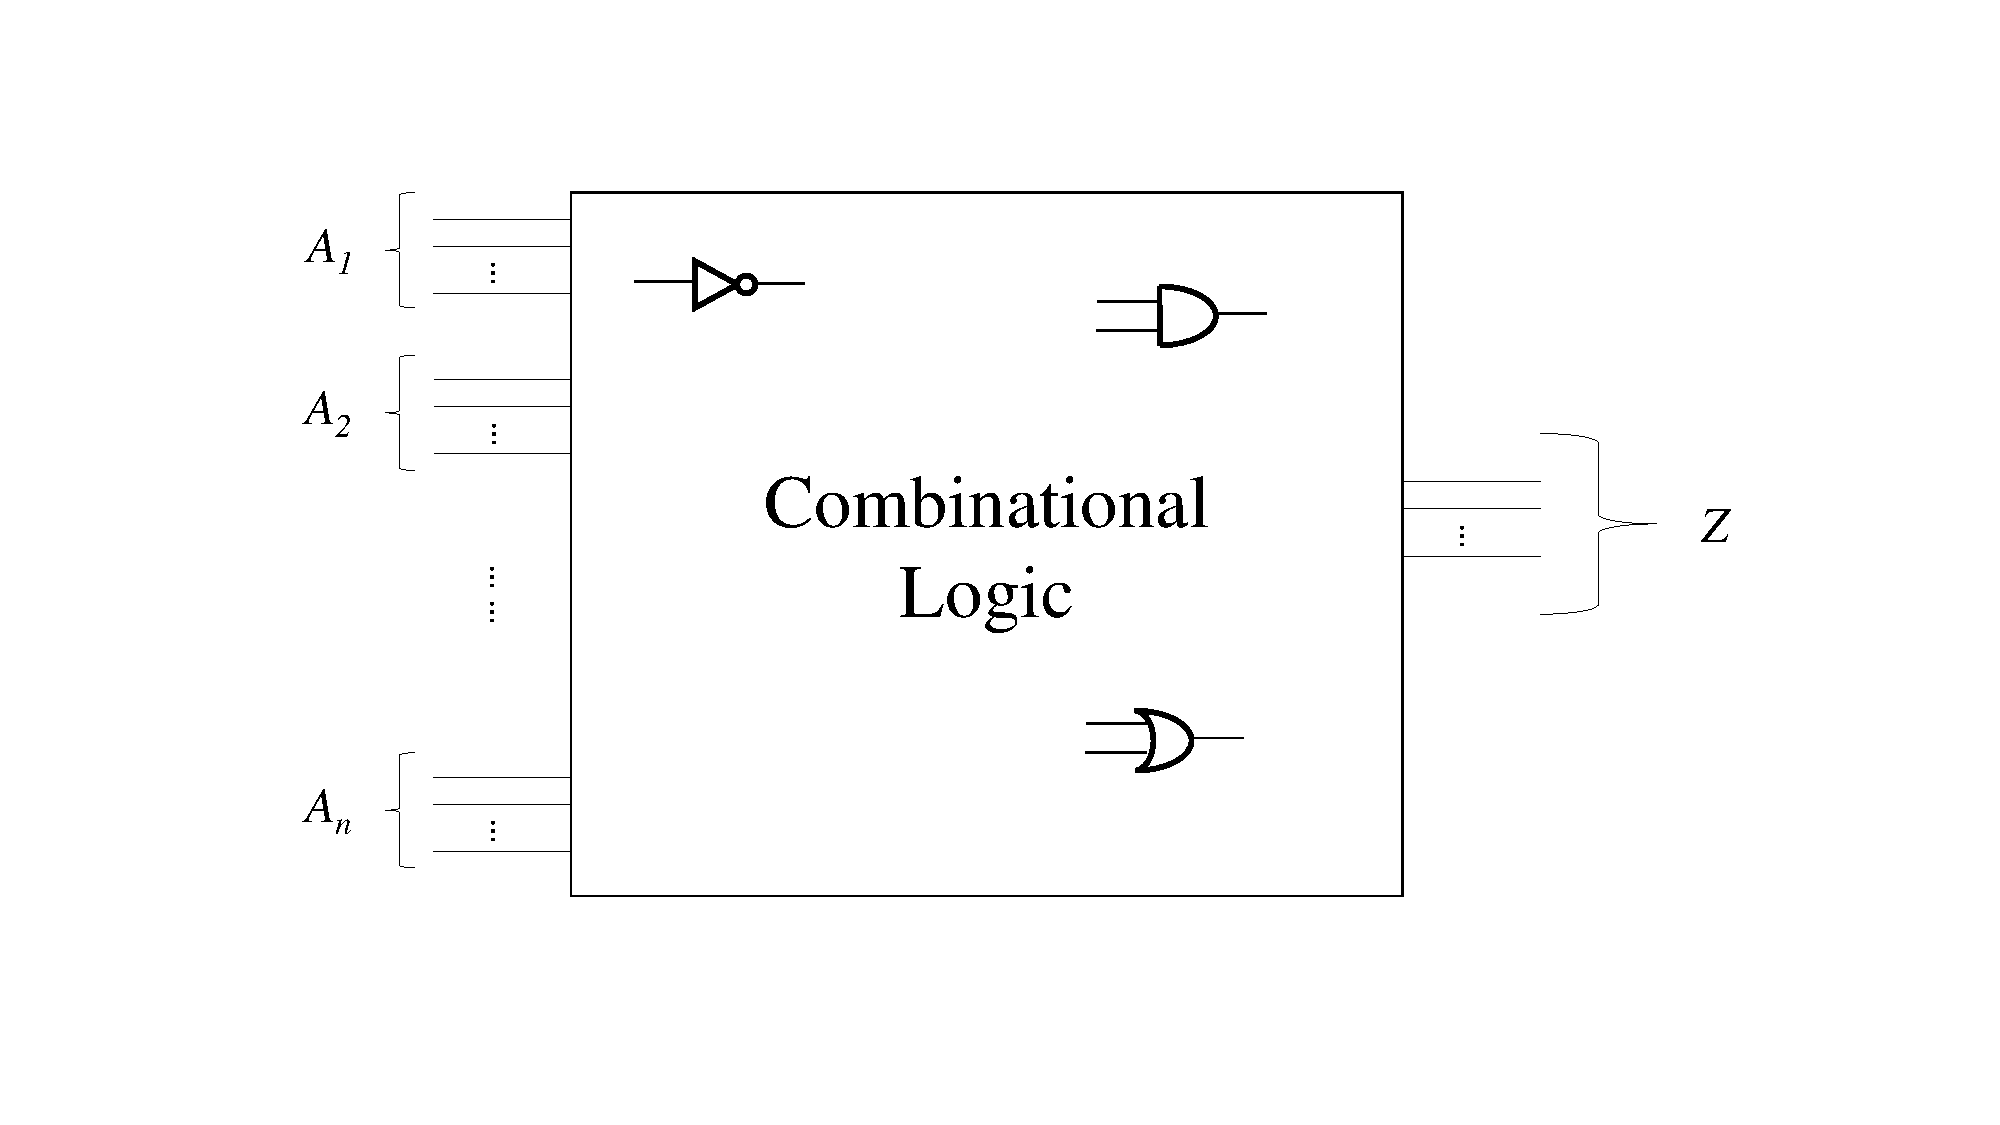
\includegraphics[width=\textwidth]{newfig/abs_setup.pdf}
\caption{Galois field arithmetic circuit model for abstraction}
\label{fig:abs_setup}}
\end{figure}

{\bf Problem setup:} Let $S$ be the system of polynomials, 
$\{f_1,\dots,f_s,f_{A_1},\dots,f_{A_n},f_{Z}\}\subset \Fkk$, 
derived from the hardware
implementation of the Galois field arithmetic circuit over $\Fkk$, as Figure \ref{fig:abs_setup} shows.
This circuit performs some unknown function $f$ over 
$\Fkk$ in the form of $Z=\Func(A_1,\dots,A_n)$, where $Z$ is the $k$-bit 
output and $A_1,\dots,A_n$ are the $k$-bit inputs.
The polynomial representation of $\Func$ over $\Fkk$ is thus:

\begin{equation}
f_{\Func}: Z+\Func(A_1,\dots,A_n) \nonumber
\end{equation}

Since $f_{\Func}$ is ultimately derived from the circuit implementation, 
it agrees with the solution to the system of polynomials $\{S\}=0$, i.e.:
\begin{equation}
f_1=\dots=f_s=f_{A_1}=\dots=f_{A_n}=f_{Z}=0 \nonumber
\end{equation}
Thus, if we let $J=\langle f_1,\dots,f_s,f_{A_1},\dots,f_{A_n},f_{Z}\rangle$ 
be the ideal generated by $S$, 
$f_{\Func}$ {\bf vanishes} on the variety $V_{\Fkk}(J)$. 
Therefore, due to Proposition \ref{pro:iofv}, 
$f_{\Func}$ must be contained in the ideal of polynomials that vanish on
this variety, $f_{\Func} \in I(V_{\Fkk}(J))$. 

By applying Strong Nullstellensatz over $\Fkk$ (Theorem \ref{thm:sns}), 
$I(V_{\Fkk}(J))=J+J_0$ where
$J_0$ is the ideal generated by all vanishing polynomials in $\Fkk$. 
Recall that a vanishing polynomial in $\Fkk[x]$ is $x^q-x=x^q+x$. 
In our case, 
$\{x_1,\dots,x_d\} \in \F_2$ and $\{A_1,\dots,A_n,Z\} \in \Fkk$.
Thus, for $\Fkk[x_1,\dots,x_d,A_1,\dots,A_n,Z]$: 
\begin{equation}
J_0 = \langle x_1^2+x_1,\dots,x_d^2+x_d, A_1^{2^k}+A_1,\dots,A_n^{2^k}+A_n,Z^{2^k}+Z\rangle \nonumber
\end{equation}

The generators of the ideal sum $J+J_0$ are simply the combination of the 
generators of $J$ and the generators $J_0$.



The variety $V_{\Fq}(J)$ is
the set of all consistent assignments to the nets (signals) in the
circuit $C$. If we {\it project this variety on the word-level input and
output variables of the circuit $C$, we essentially generate the
function $\Func$ implemented by the circuit.} Projection of varieties from
$d$-dimensional space $\Fq^d$ onto a lower dimensional subspace
$\Fq^{d-l}$ is equivalent to {\it eliminating $l$ variables} from the
corresponding ideal. This can be done by computing a \Grobner basis
of the ideal with elimination ordering, as described in the 
Elimination Theorem (Theorem \ref{thm:elimth}).
Thus, we can find the polynomial 
$f_\Func:Z+\Func(A_1,\dots,A_n)$ by computing the \Grobner
basis of $J+J_0$ using the proper elimination ordering.

The proposed elimination order for 
abstraction is defined as the {\bf abstraction term order}. 
\begin{Definition}
\label{def:ato}
Given a circuit $C$,
let $x_1, \dots, x_d$ denote all the bit-level variables, 
let $A_1,\dots,A_n$ denote the $k$-bit word-level inputs, 
and let $Z$ denote the $k$-bit word-level output. 
Using any refinement of the partial variable order 
$\{x_1, \dots, x_d\} > Z > \{A_1, \dots, A_n\}$,
% where any refinement of the order will do,
impose a lex term order $>$ on the polynomial ring 
$R = \Fq[x_1, \dots, x_d, Z, A_1, \dots, A_n]$. 
This elimination term order $>$ is defined as
the {\bf Abstraction Term Order (ATO)}. The relative ordering among $x_1,
\dots, x_d$ is not important and can be chosen arbitrarily. Likewise,
the relative ordering among $A_1, \dots, A_n$ is also unimportant.
\end{Definition}

\begin{Theorem}
{\bf Abstraction Theorem:} Using the notations from problem setup at the beginning of this subsection,
we compute a \Grobner basis $G$ of ideal $(J+J_0)$ using the abstraction term 
order $>$. Then: \\
(i) For every word-level input $A_i$, $G$ must contain the vanishing 
polynomial $A_i^q - A_i$ as the only polynomial with $A_i$ as its only 
variable;\\
(ii) $G$ must contain a polynomial of the form 
$Z + \mathcal{G}(A_1,\dots,A_n)$; and\\ 
(iii) $Z + \mathcal{G}(A_1,\dots,A_n)$ is such that 
$\Func(A_1,\dots,A_n) = {\mathcal{G}}(A_1,\dots,A_n),
\forall A_1,\dots,A_n \in \Fq$. 
In other words, ${\mathcal{G}}(A_1,\dots,A_n)$ and $\Func(A_1,\dots,A_n)$ are
equal as polynomial functions over $\Fq$.
\label{thm:abs}
\end{Theorem}

\begin{Corollary}
By computing a {\bf reduced} \Grobner basis $G_r$ of $J + J_0$, 
$G_r$ will contain one and only one polynomial in of the form 
$Z + \G(A_1,\dots,A_n)$, such that $Z = \G(A_1,\dots,A_n)$ is the 
{\bf unique, minimal, canonical} representation of the function 
$\Func$ implemented by the circuit.  
\end{Corollary}

\begin{Example}
\label{exp:finalMul2Bit}
Consider a 2-bit multiplier over ${\mathbb{F}}_{2^2}$ with
$P(x)=x^{2}+x+1$, given in Figure \ref{fig:2bitmul}. Variables $a_0,
a_1, b_0, b_1$ are primary inputs, $z_0, z_1$ are primary outputs, and
$c_0, c_1, c_2, c_3, r_0$ are intermediate variables. 
%The gate $\otimes$
%corresponds to AND-gate, i.e. bit-level multiplication modulo 2. The
%gate $\oplus$ corresponds to XOR-gate, i.e. addition modulo 2.

\begin{figure}[H]
\centerline{
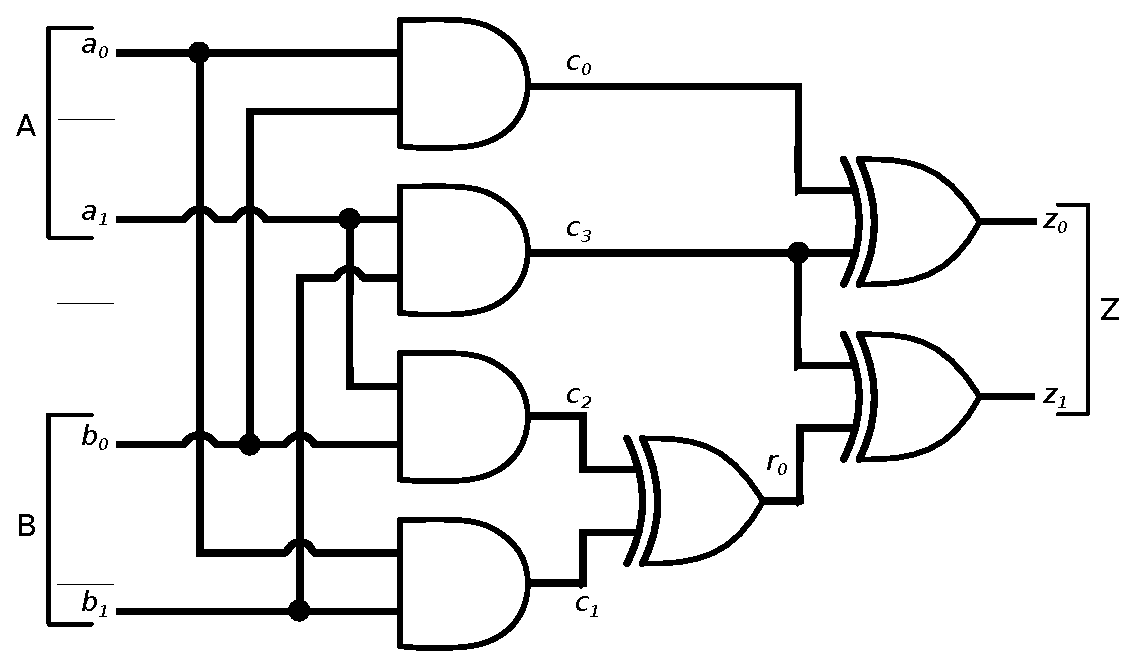
\includegraphics[scale=0.5]{./figures/2bitmasmult.eps}
}
\caption{ A 2-bit multiplier over ${\mathbb{F}}_{2^2}$.}
\label{fig:2bitmul}
\end{figure}

Polynomials extracted from the circuit implementation represent the
ideal $J$. Along with the ideal of vanishing polynomials $J_0$, 
the following polynomials represent the generators 
of $J+J_0$ for the multiplier circuit. 

\begin{eqnarray}
 \left .  
	\begin{aligned}
		f_1:c_0+a_0 \cdot b_0  \\
		f_2:c_1+a_0 \cdot b_1  \\
		f_3:c_2+a_1 \cdot b_0  \\
		f_4:c_3+a_1 \cdot b_1  \\
		f_5:r_0+c_1 + c_2		\\
		f_6:z_0+c_0 + c_3		\\
		f_7:z_1+r_0 + c_3		
	\end{aligned} 
 \ \right\}
 &\qquad&  {\it  \text{Bit-level circuit constraints} ~(\subset J)} \nonumber \\
 \left . 
	\begin{aligned}
		f_{A}:A+a_0+a_1\cdot \alpha   \\ 
		f_{B}:B+b_0+b_1\cdot \alpha  \\ 
		f_{Z}:Z+z_0+z_1\cdot \alpha   
	\end{aligned} 
 \right\}
 &\qquad&  {\it  \text{Word-level designation} ~(\subset J)} \nonumber \\
  \left . 
	\begin{aligned}
		a_0^2-a_0, ~a_1^2-a_1,~b_0^2-b_0, ~b_1^2-b_1   \\ 
		c_0^2-c_0, ~c_1^2-c_1,~c_2^2-c_2, ~c_3^2-c_3  \\ 
		r_0^2-r_0, ~z_0^2-z_0,~z_1^2-z_1    \\ 
		A^4-A, ~B^4-B ,~Z^4-Z		  
	\end{aligned} 
 \right\}
 &\qquad&  {\it \text{vanishing polynomials} (J_0)} \nonumber
\end{eqnarray}
We apply abstraction term order $>$, i.e a lex order with
"bit-level variables" $>$ "Output Z" $>$ "Inputs A, B".

When we compute the reduced \Grobner basis, $G_r$, of \{$J + J_0$\} with 
respect to this ordering, $G_r$ = \{$g_1, \dots, g_{14}\}:$
\begin{align*}
g_1: B^4+B; 
~~g_2: b_0+b_1 \alpha + B; 
~~g_3: a_0+a_1 \alpha + A;  \nonumber \\
~~g_4: c_0+c_1 \alpha + c_2 \alpha + c_3(\alpha+1)+Z;
g_5: r_0+c_1+c_2; 
~~g_6: z_0+c_0+c_3; \nonumber \\
~~g_7: z_1+r_0+c_3; 
~~{\bf g_8: Z+A\cdot B};
~~g_9: b_1+B^2+B; 
~~g_{10}: a_1+A^2+A; \nonumber \\
~~g_{11}: c_3+a_1\cdot b_1
g_{12}: c_2+a_1\cdot b_1 \alpha + a_1 \cdot B; 
~~g_{13}: c_1+a_1\cdot b_1 \alpha +b_1 A; 
~~g_{14}: A^4+A  \nonumber
\end{align*}

$g_8=Z+A\cdot B$ is the {\bf canonical, word-level polynomial } 
representing the function performed by the multiplier $Z=A\cdot B$.
\end{Example}

\section{Concluding Remarks}
Our approach to word-level abstraction of Galois field arithmetic 
circuits applies concepts of polynomial ideals, varieties, \Grobner basis, 
and abstraction theory to implement verifications on sequential circuits. 
These approaches are described in the following chapters. 